\documentclass[a4paper,12pt]{article}
\usepackage{czech}
\usepackage[utf8]{inputenc}
\usepackage{a4wide}
\usepackage[dvipdfm]{graphicx}
\usepackage{graphics}
\usepackage{indentfirst}
\usepackage{fancyhdr}
\usepackage{setspace}
\usepackage{amsmath}
\usepackage{amssymb}
\usepackage{epsfig}

\usepackage[usenames]{color}
\begin{document}

\section{Úkol}
\begin{enumerate}
	\item Změřte tuhost $k_1$ pěti pružin metoudou statickou.
	\item Sestrojte graf závislosti prodloužení pružiny na působící síle 
		$y=i(F)$
	\item Změřte tuhost $k_2$ pěti pružin metodou dynamickou.
	\item Z doby kmitu tělelsa známé hmotnosti a výchylky pružiny po 
		zavěšení tohoto tělesa určete místní tíhové zrychlení $g$.
	\item Sestrojte grafy závislostí
	\begin{enumerate}
		\item $\omega = f (\sqrt{k})$
		\item $\omega = f \left(\sqrt{\frac{1}{m}}\right)$
	\end{enumerate}
	\item Při zpracování použijte lineární regresi. 
\end{enumerate}

\section{Teorie}
\noindent
Harmocnický kmit je lineární případ pohybu, kdy se těleso pohybuje periodicky kolem jednoho bodu.
Je způsoben silou $F$, která je přímo úměrná vzdálenosti od tohoto bodu. Tato vzdálenost se 
nazývá výchylka a značí $y$. Konstanta úměrnosti se většinou značí $k$. Pohybová rovnice tedy je
\begin{eqnarray}
	F=-ky.
\end{eqnarray}

Řešení této rovnice pro okamžitou výchylku je
\begin{eqnarray}
	y=A \sin{\omega t+ \varphi},
\end{eqnarray}
kde $A$ je maximální výchylka, $\omega$ úhlová frekvence, $t$ čas a $\varphi$ počáteční fáze.
Pro úhlovou frekvecni platá vztah
\begin{eqnarray}
	\omega = \frac{2\pi}{T},
	\label{omega}
\end{eqnarray}
kde $T$ je perioda kmitu.

Pruřina se závažím $m$ v tíhovém poli je jeden z případů harmonického oscilátoru. Konstanta $k$ 
charakterizuje tuhost danné pružiny. Ta se dá určit dvěmy způsoby. 

První je statická metoda, kdy pružina nekmitá. Tíhová síla a síla, kterou působí 
pružina jsou tedy v rovnováze a platí vztah
\begin{eqnarray}
	mg=ky,
\end{eqnarray}
přičemž $y$ je výchylka od referenční polohy a $m$ hmotnost, kterou jsme na pružinu přidali.
Z tohoto snadno vyládříme vztah pro výpočet tuhosti pružiny
\begin{eqnarray}
	k=\frac{mg}{y}.
	\label{k_stat}
\end{eqnarray}

Druhá metoda, dynamická, vychází ze vztahu pro úholovou frekvecni
\begin{eqnarray}
	\omega = \sqrt{\frac{k}{m}},
	\label{omega_2}
\end{eqnarray}
kde $k$ je tuhost pružiny a $m$ hmotnost závaží na ní. Jelikož se $\omega$ špatně měřím využijeme 
vztahu \ref{omega} a nakonec vyjádříme tuhost pružiny
\begin{eqnarray}
	k=\left( \frac{2\pi}{T} \right)^2m.
	\label{k_dyn}
\end{eqnarray}

Ze studia pohybu pružiny se dá také určit tíhové zrychlení. Odvození naleznete např v \cite{text}. 
Výsledný vzorec je
\begin{eqnarray}
	g=\omega^2y_0,
	\label{g}
\end{eqnarray}
kde $y_0$ je výchylka v klidové poloze.

Bližší studium harmonického oscilátoru je v \cite{kvasnica}

\section{Výsledky měření}

\subsection{Podmínky}
\noindent
Teplota v laboratoří byla 25.1 $^{\circ}$C. Uvádím ji, protože pružiny jsou vyrobeny z kovu. Proto 
má teplota výrazný vliv na jejich rozměrym které ovlivňují jejich tuhost.

\subsection{Hmotnost závaží}
\noindent
K zatěžování pružin jsem používal sadu závaží, kde byly reprezentovány hmotnosti od pěti do sta gramů.
Pro kontrolu jejich skutečné hmotnosti jsem zvážil tři sto gramová závaží. Tato hmotnost byla
\begin{eqnarray}
	m=(299.9 \pm 0.1) \mbox{g}.
\end{eqnarray}
Chybu hmotnosti určenou tímto měřením jsem zahrnul do dalších výpočtů.

\subsection{Statická metoda}
Pro každou pružinu jsem provedl okolodeseti měření. Nejprve jsem postupně přidával sto gramová závaží 
a na závěr jsem zhustil měření v oblasti dvou set gramů. Výsledky měření jsou v tabulce \ref{stat}, kde 
veličina $y$ značí hodnotu na stupnci katetometru, u níž dolní index značí číslo pružiny. Jako nulový 
bod jsem nakonec zvolil hmotnost sto gramů, protože pružiny byly lehce zdeformované a při nižším zatížení 
se nechovali dle předpokladů. Z rozdílu hodnot $y$ jsem určil výchylku a dosadil ro rovnice \ref{k_stat}, 
přičemž od hmotnosti jsem odečetl zatížení v nulovém bodě. Výsledky naleznete v tabulce \ref{t_stat} spolu 
s jejich střední hodnotou určenou dle \cite{chyba}.

\begin{table}
$$
\begin{array}{|c|c|c|c|c|c|}
\hline
m/\mbox{g}&	y_1/\mbox{cm}&	y_2/\mbox{cm}&	y_3/\mbox{cm}&	y_4/\mbox{cm}&	y_5/\mbox{cm}	\\ \hline	
0&	44.85&	56.34&	59.73&	41.16&		\\ \hline
100&	42.16&	54.23&	35.88&	41.16&	46.66	\\ \hline
125&	41.63&	53.53&	29.68&	37.30&	45.22	\\ \hline
150&	40.92&	52.90&	24.46&	33.57&	43.85	\\ \hline
175&	39.95&	52.43&	18.80&	29.56&	42.57	\\ \hline
200&	39.38&	52.04&	13.14&	25.91&	41.40	\\ \hline
225&	38.65&	51.29&	8.18&	21.72&	40.08	\\ \hline
300&	36.72&	49.70&	&	10.56&	36.17	\\ \hline
400&	33.83&	47.75&	&	&	31.38	\\ \hline
500&	31.19&	45.64&	&	&	26.05	\\ \hline
600&	28.37&	43.31&	&	&	21.05	\\ \hline
700&	25.61&	41.23&	&	&		\\ \hline
800&	22.73&	39.21&	&	&		\\ \hline
\end{array}
$$
\caption{Výchylky pružiny při různém zatížení.}
\label{stat}
\end{table}

\begin{table}
$$
\begin{array}{|c|c|c|c|c|c|}
\hline
m/\mbox{g}&	k_1/\mbox{kg}\cdot\mbox{s}^{-2}&	k_2/\mbox{kg}\cdot\mbox{s}^{-2}&	
k_3/\mbox{kg}\cdot\mbox{s}^{-2}&	k_4/\mbox{kg}\cdot\mbox{s}^{-2}&	k_5/\mbox{kg}\cdot\mbox{s}^{-2}	\\ \hline	
125&	46.3\pm 0.2&	35.0\pm 0.1&	3.96\pm 0.02&	6.35\pm 0.03&	17.03\pm 0.07	\\ \hline
150&	39.6\pm 0.2&	36.9\pm 0.1&	4.30\pm 0.02&	6.46\pm 0.03&	17.46\pm 0.07	\\ \hline
175&	33.3\pm 0.1&	40.9\pm 0.1&	4.31\pm 0.02&	6.34\pm 0.03&	17.99\pm 0.07	\\ \hline
200&	35.3\pm 0.1&	44.8\pm 0.2&	4.31\pm 0.02&	6.43\pm 0.03&	18.65\pm 0.07	\\ \hline
225&	34.9\pm 0.1&	41.7\pm 0.1&	4.43\pm 0.03&	6.31\pm 0.04&	18.64\pm 0.07	\\ \hline
300&	36.1\pm 0.1&	43.3\pm 0.1&	&		6.41\pm 0.06&	18.70\pm 0.08	\\ \hline
400&	35.3\pm 0.1&	45.4\pm 0.2&	&		&		19.26\pm 0.08	\\ \hline
500&	35.8\pm 0.2&	45.7\pm 0.2&	&		&		19.04\pm 0.09	\\ \hline
600&	35.6\pm 0.2&	44.9\pm 0.2&	&		&		19.2\pm 0.1	\\ \hline
700&	35.6\pm 0.2&	45.3\pm 0.2&	&		&				\\ \hline
800&	35.3\pm 0.2&	45.7\pm 0.2&	&		&				\\ \hline \hline
\bar k/\mbox{kg}\cdot\mbox{s}^{-2}&		37\pm1&		43\pm1&		4.26\pm0.08&	6.38\pm 0.02&	18.4\pm0.3	\\ \hline
\end{array}
$$
\caption{Tuhost pružin pro různá zatížení určená statickou metodou.}
\label{t_stat}
\end{table}

Hodnoty z tabulky \ref{stat} jsem přepočítal na sílu působící na pružinu a za pomoci programu Gnuplot zanesl do grafu. 
Výsledný graf závislosti prodloužení na síle je obrázek \ref{g_stat}.
\begin{figure}
\begin{center}
	% GNUPLOT: LaTeX picture with Postscript
\begingroup
  \makeatletter
  \providecommand\color[2][]{%
    \GenericError{(gnuplot) \space\space\space\@spaces}{%
      Package color not loaded in conjunction with
      terminal option `colourtext'%
    }{See the gnuplot documentation for explanation.%
    }{Either use 'blacktext' in gnuplot or load the package
      color.sty in LaTeX.}%
    \renewcommand\color[2][]{}%
  }%
  \providecommand\includegraphics[2][]{%
    \GenericError{(gnuplot) \space\space\space\@spaces}{%
      Package graphicx or graphics not loaded%
    }{See the gnuplot documentation for explanation.%
    }{The gnuplot epslatex terminal needs graphicx.sty or graphics.sty.}%
    \renewcommand\includegraphics[2][]{}%
  }%
  \providecommand\rotatebox[2]{#2}%
  \@ifundefined{ifGPcolor}{%
    \newif\ifGPcolor
    \GPcolorfalse
  }{}%
  \@ifundefined{ifGPblacktext}{%
    \newif\ifGPblacktext
    \GPblacktexttrue
  }{}%
  % define a \g@addto@macro without @ in the name:
  \let\gplgaddtomacro\g@addto@macro
  % define empty templates for all commands taking text:
  \gdef\gplbacktext{}%
  \gdef\gplfronttext{}%
  \makeatother
  \ifGPblacktext
    % no textcolor at all
    \def\colorrgb#1{}%
    \def\colorgray#1{}%
  \else
    % gray or color?
    \ifGPcolor
      \def\colorrgb#1{\color[rgb]{#1}}%
      \def\colorgray#1{\color[gray]{#1}}%
      \expandafter\def\csname LTw\endcsname{\color{white}}%
      \expandafter\def\csname LTb\endcsname{\color{black}}%
      \expandafter\def\csname LTa\endcsname{\color{black}}%
      \expandafter\def\csname LT0\endcsname{\color[rgb]{1,0,0}}%
      \expandafter\def\csname LT1\endcsname{\color[rgb]{0,1,0}}%
      \expandafter\def\csname LT2\endcsname{\color[rgb]{0,0,1}}%
      \expandafter\def\csname LT3\endcsname{\color[rgb]{1,0,1}}%
      \expandafter\def\csname LT4\endcsname{\color[rgb]{0,1,1}}%
      \expandafter\def\csname LT5\endcsname{\color[rgb]{1,1,0}}%
      \expandafter\def\csname LT6\endcsname{\color[rgb]{0,0,0}}%
      \expandafter\def\csname LT7\endcsname{\color[rgb]{1,0.3,0}}%
      \expandafter\def\csname LT8\endcsname{\color[rgb]{0.5,0.5,0.5}}%
    \else
      % gray
      \def\colorrgb#1{\color{black}}%
      \def\colorgray#1{\color[gray]{#1}}%
      \expandafter\def\csname LTw\endcsname{\color{white}}%
      \expandafter\def\csname LTb\endcsname{\color{black}}%
      \expandafter\def\csname LTa\endcsname{\color{black}}%
      \expandafter\def\csname LT0\endcsname{\color{black}}%
      \expandafter\def\csname LT1\endcsname{\color{black}}%
      \expandafter\def\csname LT2\endcsname{\color{black}}%
      \expandafter\def\csname LT3\endcsname{\color{black}}%
      \expandafter\def\csname LT4\endcsname{\color{black}}%
      \expandafter\def\csname LT5\endcsname{\color{black}}%
      \expandafter\def\csname LT6\endcsname{\color{black}}%
      \expandafter\def\csname LT7\endcsname{\color{black}}%
      \expandafter\def\csname LT8\endcsname{\color{black}}%
    \fi
  \fi
  \setlength{\unitlength}{0.0500bp}%
  \begin{picture}(7200.00,5040.00)%
    \gplgaddtomacro\gplbacktext{%
      \csname LTb\endcsname%
      \put(990,440){\makebox(0,0)[r]{\strut{}-0.02}}%
      \put(990,874){\makebox(0,0)[r]{\strut{} 0}}%
      \put(990,1307){\makebox(0,0)[r]{\strut{} 0.02}}%
      \put(990,1741){\makebox(0,0)[r]{\strut{} 0.04}}%
      \put(990,2174){\makebox(0,0)[r]{\strut{} 0.06}}%
      \put(990,2608){\makebox(0,0)[r]{\strut{} 0.08}}%
      \put(990,3041){\makebox(0,0)[r]{\strut{} 0.1}}%
      \put(990,3475){\makebox(0,0)[r]{\strut{} 0.12}}%
      \put(990,3908){\makebox(0,0)[r]{\strut{} 0.14}}%
      \put(990,4342){\makebox(0,0)[r]{\strut{} 0.16}}%
      \put(990,4775){\makebox(0,0)[r]{\strut{} 0.18}}%
      \put(1122,220){\makebox(0,0){\strut{} 0}}%
      \put(1761,220){\makebox(0,0){\strut{} 5}}%
      \put(2399,220){\makebox(0,0){\strut{} 10}}%
      \put(3038,220){\makebox(0,0){\strut{} 15}}%
      \put(3676,220){\makebox(0,0){\strut{} 20}}%
      \put(4315,220){\makebox(0,0){\strut{} 25}}%
      \put(4953,220){\makebox(0,0){\strut{} 30}}%
      \put(5592,220){\makebox(0,0){\strut{} 35}}%
      \put(6230,220){\makebox(0,0){\strut{} 40}}%
      \put(6869,220){\makebox(0,0){\strut{} 45}}%
    }%
    \gplgaddtomacro\gplfronttext{%
      \csname LTb\endcsname%
      \put(5882,4602){\makebox(0,0)[r]{\strut{}"graf1.dat" u 1:2:3}}%
    }%
    \gplgaddtomacro\gplbacktext{%
      \csname LTb\endcsname%
      \put(1210,704){\makebox(0,0)[r]{\strut{}-0.02}}%
      \put(1210,1111){\makebox(0,0)[r]{\strut{} 0}}%
      \put(1210,1518){\makebox(0,0)[r]{\strut{} 0.02}}%
      \put(1210,1925){\makebox(0,0)[r]{\strut{} 0.04}}%
      \put(1210,2332){\makebox(0,0)[r]{\strut{} 0.06}}%
      \put(1210,2740){\makebox(0,0)[r]{\strut{} 0.08}}%
      \put(1210,3147){\makebox(0,0)[r]{\strut{} 0.1}}%
      \put(1210,3554){\makebox(0,0)[r]{\strut{} 0.12}}%
      \put(1210,3961){\makebox(0,0)[r]{\strut{} 0.14}}%
      \put(1210,4368){\makebox(0,0)[r]{\strut{} 0.16}}%
      \put(1210,4775){\makebox(0,0)[r]{\strut{} 0.18}}%
      \put(1342,484){\makebox(0,0){\strut{} 0}}%
      \put(1956,484){\makebox(0,0){\strut{} 5}}%
      \put(2570,484){\makebox(0,0){\strut{} 10}}%
      \put(3184,484){\makebox(0,0){\strut{} 15}}%
      \put(3798,484){\makebox(0,0){\strut{} 20}}%
      \put(4413,484){\makebox(0,0){\strut{} 25}}%
      \put(5027,484){\makebox(0,0){\strut{} 30}}%
      \put(5641,484){\makebox(0,0){\strut{} 35}}%
      \put(6255,484){\makebox(0,0){\strut{} 40}}%
      \put(6869,484){\makebox(0,0){\strut{} 45}}%
      \put(308,2739){\rotatebox{-270}{\makebox(0,0){\strut{}bla}}}%
      \put(4105,154){\makebox(0,0){\strut{}blx}}%
    }%
    \gplgaddtomacro\gplfronttext{%
      \csname LTb\endcsname%
      \put(5882,4602){\makebox(0,0)[r]{\strut{}"graf1.dat" u 1:2:3}}%
    }%
    \gplbacktext
    \put(0,0){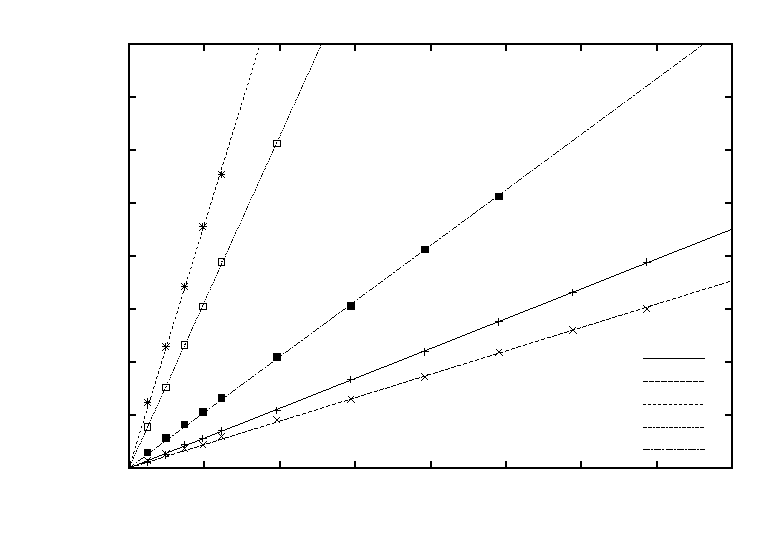
\includegraphics{graf1}}%
    \gplfronttext
  \end{picture}%
\endgroup

\end{center}
	\caption{Graf závislosti prodloužení na působící síle}
	\label{g_stat}
\end{figure}

\subsection{Dynamická metoda}
\noindent
Periodu kmitů pružiny jsem určival spolu s výchylkou ve statické poloze, abych zkráteil dobu měření. 
Změřil jsem vždy dobu dvaceti kmitů pružiny pro každou hmotnost. Měření jsem provedl dvakrát, abych vyloučil hrubou 
chybu. Stopky sice meřili s přesností na dvě desetinná místa, ale vzhledem k reakčí době 0.2 s, se kterou jsem počítal 
jsem hodnoty zaokrouhlil. Naměřeně časy jsou v tabulce \ref{dyn_T}.

\begin{table}
$$
\begin{array}{|c|c|c|c|c|c|}
\hline
m/\mbox{g}&	20\cdot T_1/\mbox{cm}&	20\cdot T_2/\mbox{cm}&	20\cdot T_3/\mbox{cm}&	20\cdot T_4/\mbox{cm}&	20\cdot T_5/\mbox{cm}	\\ \hline	
125&	7.9&	6.6&	21.2&	17.7&	10.1	\\ \hline
150&	8.6&	7.2&	23.0&	19.4&	11.2	\\ \hline
175&	9.3&	7.8&	24.6&	20.9&	12.0	\\ \hline
200&	9.8&	8.3&	25.5&	22.1&	12.8	\\ \hline
225&	10.4&	8.8&	27.0&	23.5&	13.6	\\ \hline
300&	11.9&	10.1&	&	26.8&	15.7	\\ \hline
400&	13.7&	11.6&	&	&	18.1	\\ \hline
500&	15.2&	12.9&	&	&	20.2	\\ \hline
600&	16.6&	14.0&	&	&	22.1	\\ \hline
700&	17.9&	15.0&	&	&		\\ \hline
800&	19.1&	15.8&	&	&		\\ \hline
\end{array}
$$
\caption{Doba dvaceti kmitů pružiny pro různé zatížení pružin.}
\label{dyn_T}
\end{table}

Výsledky jsem dále dosadil do vztahu \ref{k_dyn} a vypočetl ruhost pružiny $k$. Výsledky jsou shrnuty v tabulce \ref{dyn_k} 
opět s vypočítanou střední hodnotou.

\begin{table}
$$
\begin{array}{|c|c|c|c|c|c|}
\hline
m/\mbox{g}&	k_1/\mbox{kg}\cdot\mbox{s}^{-2}&	k_2/\mbox{kg}\cdot\mbox{s}^{-2}&	k_3/\mbox{kg}\cdot\mbox{s}^{-2}&	k_4/\mbox{kg}\cdot\mbox{s}^{-2}&	k_5/\mbox{kg}\cdot\mbox{s}^{-2}	\\ \hline	
125&	31.6\pm 0.2&	45.3\pm 0.2&	4.39\pm 0.07&	6.30\pm 0.08&	19.4\pm 0.1	\\ \hline
150&	32.0\pm 0.2&	45.7\pm 0.2&	4.48\pm 0.08&	6.29\pm 0.09&	18.9\pm 0.2	\\ \hline
175&	32.0\pm 0.2&	45.4\pm 0.3&	4.57\pm 0.08&	6.33\pm 0.10&	19.2\pm 0.2	\\ \hline
200&	32.9\pm 0.2&	45.8\pm 0.3&	4.86\pm 0.09&	6.4\pm 0.1&	19.3\pm 0.2	\\ \hline
225&	32.9\pm 0.3&	45.9\pm 0.3&	4.87\pm 0.10&	6.4\pm 0.1&	19.2\pm 0.2	\\ \hline
300&	33.5\pm 0.3&	46.4\pm 0.4&		&	6.6\pm 0.1&	19.2\pm 0.2	\\ \hline
400&	33.7\pm 0.3&	46.9\pm 0.4&		&	&		19.3\pm 0.3	\\ \hline
500&	34.2\pm 0.4&	47.4\pm 0.5&		&	&		19.4\pm 0.3	\\ \hline
600&	34.4\pm 0.4&	48.3\pm 0.5&		&	&		19.4\pm 0.3	\\ \hline
700&	34.5\pm 0.5&	49.1\pm 0.6&		&	&				\\ \hline
800&	34.6\pm 0.5&	50.6\pm 0.6&		&	&				\\ \hline
\bar k/\mbox{kg}\cdot\mbox{s}^{-2}&	33.3\pm 0.3&	47.0\pm 0.5&	4.63\pm 0.10&	6.39\pm 0.05&	19.26\pm 0.05 \\ \hline		
\end{array}
$$
\caption{Hodnoty $k$ určené dynamickou metodou.}
\label{dyn_k}
\end{table}

\subsection{Tíhové zrychlení}
\noindent
Hodnoty z tabulek \ref{stat} a \ref{dyn_T} jsem dosadil od vzorců \ref{omega} a \ref{g}. Tyto hodnoty jsem následné 
statisticky vyhodnotil dle \cite{chyba}. Byl jsem nucen zanedbat hodnoty, které zjevně neodpovídali skutečnosti, 
protože předevšim u větších pružin byl vzorec pro výpočet $g$ chybný.  Výsledné tíhové zrychlení jsem stanovil na
\begin{eqnarray}
	g=(9.7\pm0.2)\mbox{m}\cdot\mbox{s}^{-2}
\end{eqnarray}

\subsection{Grafy závislost $\omega$}
\noindent
Dle hodnot z tabulek výše jsem za pomoci programu gnuplot sestrojil grafy závislosti $\omega$ na $\sqrt{k}$ resp. 
$\sqrt{\frac{1}{m}}$, které jsou obrázky \ref{graf2} resp. \ref{graf3}.

\begin{figure}
\begin{center}
	% GNUPLOT: LaTeX picture with Postscript
\begingroup
  \makeatletter
  \providecommand\color[2][]{%
    \GenericError{(gnuplot) \space\space\space\@spaces}{%
      Package color not loaded in conjunction with
      terminal option `colourtext'%
    }{See the gnuplot documentation for explanation.%
    }{Either use 'blacktext' in gnuplot or load the package
      color.sty in LaTeX.}%
    \renewcommand\color[2][]{}%
  }%
  \providecommand\includegraphics[2][]{%
    \GenericError{(gnuplot) \space\space\space\@spaces}{%
      Package graphicx or graphics not loaded%
    }{See the gnuplot documentation for explanation.%
    }{The gnuplot epslatex terminal needs graphicx.sty or graphics.sty.}%
    \renewcommand\includegraphics[2][]{}%
  }%
  \providecommand\rotatebox[2]{#2}%
  \@ifundefined{ifGPcolor}{%
    \newif\ifGPcolor
    \GPcolorfalse
  }{}%
  \@ifundefined{ifGPblacktext}{%
    \newif\ifGPblacktext
    \GPblacktexttrue
  }{}%
  % define a \g@addto@macro without @ in the name:
  \let\gplgaddtomacro\g@addto@macro
  % define empty templates for all commands taking text:
  \gdef\gplbacktext{}%
  \gdef\gplfronttext{}%
  \makeatother
  \ifGPblacktext
    % no textcolor at all
    \def\colorrgb#1{}%
    \def\colorgray#1{}%
  \else
    % gray or color?
    \ifGPcolor
      \def\colorrgb#1{\color[rgb]{#1}}%
      \def\colorgray#1{\color[gray]{#1}}%
      \expandafter\def\csname LTw\endcsname{\color{white}}%
      \expandafter\def\csname LTb\endcsname{\color{black}}%
      \expandafter\def\csname LTa\endcsname{\color{black}}%
      \expandafter\def\csname LT0\endcsname{\color[rgb]{1,0,0}}%
      \expandafter\def\csname LT1\endcsname{\color[rgb]{0,1,0}}%
      \expandafter\def\csname LT2\endcsname{\color[rgb]{0,0,1}}%
      \expandafter\def\csname LT3\endcsname{\color[rgb]{1,0,1}}%
      \expandafter\def\csname LT4\endcsname{\color[rgb]{0,1,1}}%
      \expandafter\def\csname LT5\endcsname{\color[rgb]{1,1,0}}%
      \expandafter\def\csname LT6\endcsname{\color[rgb]{0,0,0}}%
      \expandafter\def\csname LT7\endcsname{\color[rgb]{1,0.3,0}}%
      \expandafter\def\csname LT8\endcsname{\color[rgb]{0.5,0.5,0.5}}%
    \else
      % gray
      \def\colorrgb#1{\color{black}}%
      \def\colorgray#1{\color[gray]{#1}}%
      \expandafter\def\csname LTw\endcsname{\color{white}}%
      \expandafter\def\csname LTb\endcsname{\color{black}}%
      \expandafter\def\csname LTa\endcsname{\color{black}}%
      \expandafter\def\csname LT0\endcsname{\color{black}}%
      \expandafter\def\csname LT1\endcsname{\color{black}}%
      \expandafter\def\csname LT2\endcsname{\color{black}}%
      \expandafter\def\csname LT3\endcsname{\color{black}}%
      \expandafter\def\csname LT4\endcsname{\color{black}}%
      \expandafter\def\csname LT5\endcsname{\color{black}}%
      \expandafter\def\csname LT6\endcsname{\color{black}}%
      \expandafter\def\csname LT7\endcsname{\color{black}}%
      \expandafter\def\csname LT8\endcsname{\color{black}}%
    \fi
  \fi
  \setlength{\unitlength}{0.0500bp}%
  \begin{picture}(11904.00,8502.00)%
    \gplgaddtomacro\gplbacktext{%
      \csname LTb\endcsname%
      \put(1474,1894){\makebox(0,0)[r]{\strut{} 0,003}}%
      \put(1474,3380){\makebox(0,0)[r]{\strut{} 0,0035}}%
      \put(1474,4867){\makebox(0,0)[r]{\strut{} 0,004}}%
      \put(1474,6354){\makebox(0,0)[r]{\strut{} 0,0045}}%
      \put(1474,7841){\makebox(0,0)[r]{\strut{} 0,005}}%
      \put(2515,484){\makebox(0,0){\strut{} 0,1}}%
      \put(5534,484){\makebox(0,0){\strut{} 1}}%
      \put(8554,484){\makebox(0,0){\strut{} 10}}%
      \put(11573,484){\makebox(0,0){\strut{} 100}}%
      \put(308,4272){\rotatebox{-270}{\makebox(0,0){\strut{}\rotatebox{-90}{$\frac{1/T}{\mathrm{K^{-1}}}$}}}}%
      \put(6589,154){\makebox(0,0){\strut{}$\frac{R}{\mathrm k\Omega}$}}%
      \put(6589,8171){\makebox(0,0){\strut{}Graf 2: Z\'avislost odporu na p\v{r}evr\'acen\'e hodnot\v{e} teploty}}%
    }%
    \gplgaddtomacro\gplfronttext{%
      \csname LTb\endcsname%
      \put(5302,7668){\makebox(0,0)[r]{\strut{}$R(1/T)$}}%
      \csname LTb\endcsname%
      \put(5302,7448){\makebox(0,0)[r]{\strut{}Prolo\v{z}en\'a z\'avislost}}%
    }%
    \gplbacktext
    \put(0,0){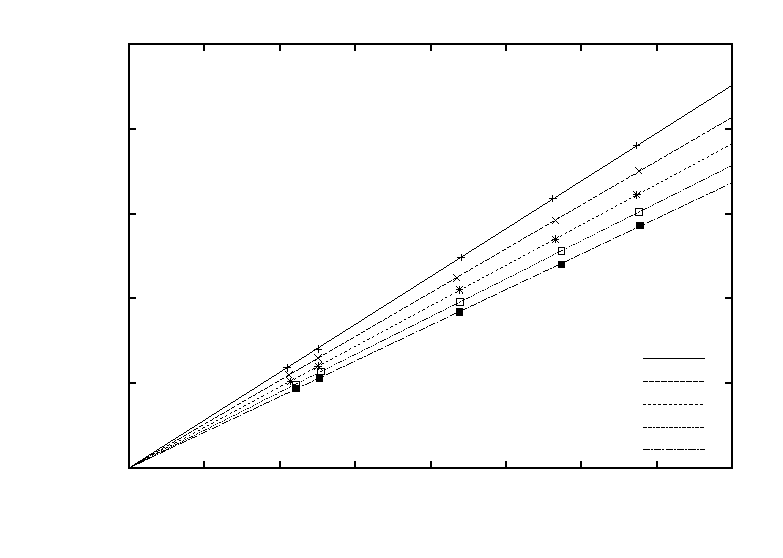
\includegraphics{graf2}}%
    \gplfronttext
  \end{picture}%
\endgroup

\end{center}
	\caption{Graf závislosti $\omega$ na $\sqrt{k}$}
	\label{graf2}
\end{figure}

\begin{figure}
\begin{center}
	% GNUPLOT: LaTeX picture with Postscript
\begingroup
  \makeatletter
  \providecommand\color[2][]{%
    \GenericError{(gnuplot) \space\space\space\@spaces}{%
      Package color not loaded in conjunction with
      terminal option `colourtext'%
    }{See the gnuplot documentation for explanation.%
    }{Either use 'blacktext' in gnuplot or load the package
      color.sty in LaTeX.}%
    \renewcommand\color[2][]{}%
  }%
  \providecommand\includegraphics[2][]{%
    \GenericError{(gnuplot) \space\space\space\@spaces}{%
      Package graphicx or graphics not loaded%
    }{See the gnuplot documentation for explanation.%
    }{The gnuplot epslatex terminal needs graphicx.sty or graphics.sty.}%
    \renewcommand\includegraphics[2][]{}%
  }%
  \providecommand\rotatebox[2]{#2}%
  \@ifundefined{ifGPcolor}{%
    \newif\ifGPcolor
    \GPcolorfalse
  }{}%
  \@ifundefined{ifGPblacktext}{%
    \newif\ifGPblacktext
    \GPblacktexttrue
  }{}%
  % define a \g@addto@macro without @ in the name:
  \let\gplgaddtomacro\g@addto@macro
  % define empty templates for all commands taking text:
  \gdef\gplbacktext{}%
  \gdef\gplfronttext{}%
  \makeatother
  \ifGPblacktext
    % no textcolor at all
    \def\colorrgb#1{}%
    \def\colorgray#1{}%
  \else
    % gray or color?
    \ifGPcolor
      \def\colorrgb#1{\color[rgb]{#1}}%
      \def\colorgray#1{\color[gray]{#1}}%
      \expandafter\def\csname LTw\endcsname{\color{white}}%
      \expandafter\def\csname LTb\endcsname{\color{black}}%
      \expandafter\def\csname LTa\endcsname{\color{black}}%
      \expandafter\def\csname LT0\endcsname{\color[rgb]{1,0,0}}%
      \expandafter\def\csname LT1\endcsname{\color[rgb]{0,1,0}}%
      \expandafter\def\csname LT2\endcsname{\color[rgb]{0,0,1}}%
      \expandafter\def\csname LT3\endcsname{\color[rgb]{1,0,1}}%
      \expandafter\def\csname LT4\endcsname{\color[rgb]{0,1,1}}%
      \expandafter\def\csname LT5\endcsname{\color[rgb]{1,1,0}}%
      \expandafter\def\csname LT6\endcsname{\color[rgb]{0,0,0}}%
      \expandafter\def\csname LT7\endcsname{\color[rgb]{1,0.3,0}}%
      \expandafter\def\csname LT8\endcsname{\color[rgb]{0.5,0.5,0.5}}%
    \else
      % gray
      \def\colorrgb#1{\color{black}}%
      \def\colorgray#1{\color[gray]{#1}}%
      \expandafter\def\csname LTw\endcsname{\color{white}}%
      \expandafter\def\csname LTb\endcsname{\color{black}}%
      \expandafter\def\csname LTa\endcsname{\color{black}}%
      \expandafter\def\csname LT0\endcsname{\color{black}}%
      \expandafter\def\csname LT1\endcsname{\color{black}}%
      \expandafter\def\csname LT2\endcsname{\color{black}}%
      \expandafter\def\csname LT3\endcsname{\color{black}}%
      \expandafter\def\csname LT4\endcsname{\color{black}}%
      \expandafter\def\csname LT5\endcsname{\color{black}}%
      \expandafter\def\csname LT6\endcsname{\color{black}}%
      \expandafter\def\csname LT7\endcsname{\color{black}}%
      \expandafter\def\csname LT8\endcsname{\color{black}}%
    \fi
  \fi
  \setlength{\unitlength}{0.0500bp}%
  \begin{picture}(11904.00,8502.00)%
    \gplgaddtomacro\gplbacktext{%
      \csname LTb\endcsname%
      \put(1342,704){\makebox(0,0)[r]{\strut{} 0}}%
      \put(1342,1554){\makebox(0,0)[r]{\strut{} 0,005}}%
      \put(1342,2403){\makebox(0,0)[r]{\strut{} 0,01}}%
      \put(1342,3253){\makebox(0,0)[r]{\strut{} 0,015}}%
      \put(1342,4103){\makebox(0,0)[r]{\strut{} 0,02}}%
      \put(1342,4952){\makebox(0,0)[r]{\strut{} 0,025}}%
      \put(1342,5802){\makebox(0,0)[r]{\strut{} 0,03}}%
      \put(1342,6652){\makebox(0,0)[r]{\strut{} 0,035}}%
      \put(1342,7501){\makebox(0,0)[r]{\strut{} 0,04}}%
      \put(1474,484){\makebox(0,0){\strut{} 0}}%
      \put(2917,484){\makebox(0,0){\strut{} 100}}%
      \put(4359,484){\makebox(0,0){\strut{} 200}}%
      \put(5802,484){\makebox(0,0){\strut{} 300}}%
      \put(7245,484){\makebox(0,0){\strut{} 400}}%
      \put(8688,484){\makebox(0,0){\strut{} 500}}%
      \put(10130,484){\makebox(0,0){\strut{} 600}}%
      \put(11573,484){\makebox(0,0){\strut{} 700}}%
      \put(308,4272){\rotatebox{-270}{\makebox(0,0){\strut{}\rotatebox{-90}{$\frac{UI}{\mathrm{W}}$}}}}%
      \put(6523,154){\makebox(0,0){\strut{}$\frac{U/I}{\Omega}$}}%
      \put(6523,8171){\makebox(0,0){\strut{}Graf 3: Z\'avislost v\'ykonu na odporu}}%
    }%
    \gplgaddtomacro\gplfronttext{%
      \csname LTb\endcsname%
      \put(10586,7668){\makebox(0,0)[r]{\strut{}$P(R)$}}%
      \csname LTb\endcsname%
      \put(10586,7448){\makebox(0,0)[r]{\strut{}Prolo\v{z}en\'a z\'vislost}}%
    }%
    \gplbacktext
    \put(0,0){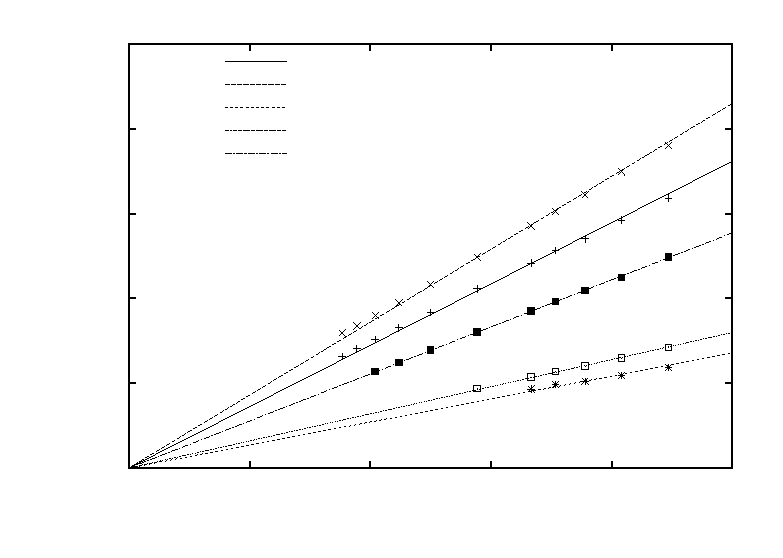
\includegraphics{graf3}}%
    \gplfronttext
  \end{picture}%
\endgroup

\end{center}
	\caption{Graf závislosti $\omega$ na $\sqrt{\frac{1}{m}}$}
	\label{graf3}
\end{figure}

\section{Diskuze}
\noindent
Ukázalo se, že přesnost určení tuhosti statickou metodou velmi závisí na délce a hustotě závitů. Velká 
pružina (číslo 1) měla při nižším zatížení velmi rozdílné parametry. Dynamická metoda tak náchylná nebyla. 

Tíhové zrychlení určené za pomoci pružiny vcelku odpovídá realitě, akorát jsem byl nuce vynechat spoustu 
hodnot. Jednalo se především o ty větších pružin za nízkého zatížení.

U dynamické metody bylo opět u nižích závaží, protože perioda byla velmi krátká a i dvacet kmitů nebylo 
vzhledem k chybě dostačující. Více jsem jich však měřit nemohl, protože osa kmitu se s časem vychylovala 
a místí byla její precese tak veliká, že ani dvacet kmitůneporběhlo správně.

Výsledné grafy vyšli dle mého nározu dobře. Chyba fitu nebyla vysoká. Dokonce nedosáhla ani celého procenta.

\section{Závěr}
\noindent
Určil jsem tuhost pružin $k$, které jsou shrnuty v tabulce \ref{t_stat}. \\
Sestrojil jsem graf závislosti prodloužení na působící síle, který je na obrázku \ref{g_stat}. \\
Určil jsem tuhost pružin $k$ dynamickou metodou shrnuté v tabulce \ref{dyn_k}.\\
Z doby kmitu jsem snanovil hodnotu tíhového zrychlení
\begin{eqnarray}
	g=(9.7\pm0.2)\mbox{m}\cdot\mbox{s}^{-2}.
\end{eqnarray}
Sestrojil jsem grafy závislosti $\omega$ dle zadání. Jedná se o obrázky \ref{graf2} a \ref{graf3}.

\eject
\begin{thebibliography}{5}
        \bibitem{text} \textbf{Studijní text na praktikum I} \\http://physics.mff.cuni.cz/vyuka/zfp/txt\_102.pdf (16. 4. 2011)
        \bibitem{kvasnica} \emph{Prof. RNDr. Jozef Kvasnica, DrSc. a kolektiv}: \textbf{Mechanika}\\ Academia, Praha 1988
        \bibitem{chyba} \emph{J. Englich}: \textbf{Zpracování výsldků fyzikálních měření} \\ LS 1999/2000
\end{thebibliography}

\end{document}
